\documentclass{dmgt}
%
\usepackage{graphicx} % Required for inserting images
\usepackage[T1]{fontenc}
\usepackage[latin9]{inputenc}
\usepackage{float}
\restylefloat{figure}
\usepackage{amsmath}
\usepackage{amsthm}
\usepackage{amssymb}
\usepackage{wasysym}
\usepackage{pdfpages}
\usepackage{verbatim}
\usepackage{multirow}
\usepackage{tikz}
\usepackage{caption}
\usepackage{subcaption}
\usepackage{placeins}
%\usepackage{subfig}
\usepackage{amsfonts}
\usepackage{standalone}
\usepackage{multicol}
\usepackage{lineno}
\usepackage{hyperref}
%\usepackage[export]{adjustbox}
%
\usepackage{tikz}
\usepackage{tikz-network}
\usetikzlibrary{shapes}
\usetikzlibrary{calc}
\usetikzlibrary{positioning}
\tikzstyle{vertex}=[circle, draw, inner sep=2pt, minimum size=6pt]
\newcommand{\vertex}{\node[vertex]}

%%% Commands for Common Mathematical Fields and Number Sets
\newcommand{\kk}{\ensuremath{\Bbbk}} % Generic field symbol
\newcommand{\CC}{\ensuremath{\mathbb{C}}} % Complex numbers
\newcommand{\FF}{\ensuremath{\mathbb{F}}} % Field
\newcommand{\NN}{\ensuremath{\mathbb{N}}} % Natural numbers
\newcommand{\QQ}{\ensuremath{\mathbb{Q}}} % Rational numbers
\newcommand{\RR}{\ensuremath{\mathbb{R}}} % Real numbers
\newcommand{\ZZ}{\ensuremath{\mathbb{Z}}} % Integers

%%% Commands for Common Mathematical Sets and Spaces
\newcommand{\MM}{\ensuremath{\mathcal{M}}} % Set of matrices
\newcommand{\TT}{\ensuremath{\mathcal{T}}} % Topological space
\newcommand{\BB}{\ensuremath{\mathcal{B}}} % Basis or perhaps block
\newcommand{\VV}{\ensuremath{\mathcal{V}}} % Vector space
\newcommand{\WW}{\ensuremath{\mathcal{W}}} % Another vector space
\newcommand{\UU}{\ensuremath{\mathcal{U}}} % Another vector space
\newcommand{\PP}{\ensuremath{\mathcal{P}}} % Power set
\newcommand{\GG}{\ensuremath{\mathcal{G}}} % fancy G

\usepackage{graphicx}
\usepackage{array}
\usepackage{standalone}
\usepackage{amsmath}
\usepackage{xtab}
\usepackage{longtable} % Force consistent column widths across pages

%% do not change the next command
%% \setarticle{1}{xx}{yyyy}

\newauthor{%
Daniel Banegas}{%
D. Banegas }{%
University of Minnesota Duluth\\
Duluth, MN, USA}[%
baneg003@d.umn.edu]

\newauthor{%
Bryan Freyberg}{%
B. Freyberg}{%
University of Minnesota Duluth\\
Duluth, MN, USA}[%
frey0031@d.umn.edu]

\title{Decomposition of complete graphs into forests with seven edges}

\keywords{Graph decomposition, forests, $\rho$-labeling}

\classnbr{05C51}

\begin{document}
\begin{abstract}
 Let $K$ be a graph and $G$ a subgraph of $K$. If $E(K)$ can be partitioned into edge-disjoint copies of $G$, we call the partition a $G$-decomposition of $K$ and say that $G$ decomposes $K.$ There are 47 forests with exactly 7 edges. We prove that every one decomposes the complete graph $K_{n}$ if and only if $n \equiv 0 \textrm{ or }1\pmod{7}.$
\end{abstract}
%%%%%%%%%%%5
\section{Introduction}
A \textit{$G$-decomposition} of a graph $K$ is a set of mutually edge-disjoint subgraphs of $K$ which are isomorphic to a given graph $G$. If such a set exists we say that $K$ \textit{allows} a $G$-decomposition, and if $K\cong K_{n}$ we sometimes call the decomposition a \textit{$G$-design of order $n$}.

$G$-decompositions are a longstanding topic in combinatorics, graph theory, and design theory, with roots tracing back to at least the 19th century. The work of Rosa and Kotzig in the 1960s on what are now known as graph labelings laid the foundation for the modern treatment of such problems. Using adaptations of these labelings alongside techniques from design theory, numerous papers have since been published on $G$-decompositions. This work is a natural continuation of Freyberg and Peters' recent paper on decomposing complete graphs into forests with six edges \cite{bib:Peters}. Their paper also includes a summary of $G$-decompositions for graphs $G$ with less than 7 edges.

Every connected component of a forest with 7 edges is a tree with 6 or less edges. All such trees are cataloged in Figure \ref{fig:catalog}. We use the naming convention $\mathbf{T_{j}^i}$ to denote the $i^{\textrm{th}}$ tree with $j$ vertices. For each tree $\mathbf{T_{j}^i}$, the names of the vertices, $v_t$ for $1 \leq t \leq j,$ will be referred to in the decompositions described in Section \ref{sec:7 or 8 mod 14}.

\begin{figure}[]
\centering
    \includegraphics{tree chart.pdf}
    \caption{Trees with less than 7 edges}
    \label{fig:catalog}
\end{figure}
The next theorem gives the necessary conditions for the existence of a $G$-decomposition of $K_n$ when $G$ is a graph with 7 edges.

\begin{theorem}
  If $G$ is a graph with $7$ edges and a $G$-decomposition of $K_n$ exists, then $n \equiv 0,1,7, \textrm{or} \; 8 \pmod{14}.$  
\end{theorem}
\begin{proof}
    If a $G$-decomposition exists, then $7 | \binom{n}{2}$ which immediately implies $n \equiv 0,1,7, \textrm{or} \; 8 \pmod{14}.$
\end{proof}

In this article, we only consider simple graphs without isolated vertices. There are $47$ non-isomorphic forests with $7$ edges. Section \ref{sec:0 or 1 mod 14} treats all $47$ forests when $n \equiv 0 \textrm{ or } 1 \pmod{14}$. Section \ref{sec:7 or 8 mod 14} applies to all the forests when $n \equiv 7 \textrm{ or } 8 \pmod{14}$ with the lone exception of $F \cong \mathbf{T_{7}^{11}}\sqcup\mathbf{T_{2}^{1}},$ which  is solved for those values of $n$ in Section \ref{sec:star}. 
%%%%%%%%%%%%%%%%%%%%%%%%%%%%%%%%%%%%%%%%%
%figure 1 shows up here
\section{$n \equiv 0 \textrm{ or } 1 \pmod{14}$}\label{sec:0 or 1 mod 14}

In this section, we use established graph labeling techniques to construct the $G$-decompositions of $K_n$ when $n \equiv 0 \textrm{ or } 1 \pmod{14}$. 



\begin{dnt}[(Rosa \cite{bib:rosa})] \label{def:rho} 
 Let $G$ be a graph with $m$ edges.  A \textit{$\rho$-labeling} of $G$ is an injection $f: V(G) \rightarrow \{0,1,2, \dots, 2m\}$ that induces a bijective \textit{length function $\ell: E(G) \rightarrow \{1,2, \dots, m\}$} where 
    $$
    \ell(uv) = \text{min}\{|f(u)-f(v)|,2m+1-|f(u)-f(v)|\},
    $$
for all  $uv \in E(G)$.
\end{dnt}

Rosa showed that a $\rho$-labeling of a graph $G$ with $m$ edges and a cyclic $G$-decomposition of $K_{2m+1}$ are equivalent, which the next theorem shows. Later, Rosa, his students, and colleagues began considering more restrictive types of $\rho$-labeling to address decomposing complete graphs of more orders. Definitions of these labelings and related results follow.

\begin{theorem}[(Rosa \cite{bib:rosa})]\label{thm:Rhosa}  
Let $G$ be a graph with $m$ edges.  There exists a cyclic $G$-decomposition of $K_{2m+1}$ if and only if $G$ admits a $\rho$-labeling.
\end{theorem}

\begin{dnt}[(Rosa \cite{bib:rosa})] \label{def:sigma} 
A $\sigma$-labeling of a graph $G$ is a $\rho$-labeling such that $\ell(uv) = |f(u) - f(v)|$ for all $uv \in E(G).$
\end{dnt}

\begin{dnt}[(El-Zanati, Vanden Eynden \cite{cyclicbipart})] \label{def:rho and sigma ordered def} 
A $\rho$- or $\sigma$-labeling of a bipartite graph $G$ with bipartition $(A,B)$ is called an \emph{ordered} $\rho$- or $\sigma$-labeling and denoted $\rho^+,\sigma^+$, respectively, if $f(a) < f(b)$ for each edge $ab$ with $a \in A$ and $b \in B$.
\end{dnt}

\begin{theorem}[(El-Zanati, Vanden Eynden \cite{cyclicbipart})] \label{thm:rho plus} 
Let $G$ be a graph with $m$ edges which has a $\rho^+$-labeling.  Then $G$ decomposes $K_{2mk+1}$ for all positive integers $k$.
\end{theorem}

\begin{dnt}[(Freyberg, Tran \cite{tran})] \label{def:sigma plus minus} 
A $\sigma^{+-}$-\emph{labeling} of a bipartite graph $G$ with $m$ edges and bipartition $(A,B)$ is a $\sigma^+$-labeling with the property that $f(a) - f(b) \neq m$ for all $a \in A$ and $b \in B$, and $f(v) \not\in \{2m,2m-1\}$ for any $v\in V(G)$.
\end{dnt}

\begin{theorem}[(Freyberg, Tran \cite{tran})] \label{thm:sigma plus minus} 
Let $G$ be a graph with $m$ edges and a $\sigma^{+-}$-labeling such that the edge of length $m$ is a pendant. Then there exists a $G$-decomposition of both $K_{2mk}$ and $K_{2mk+1}$ for every positive integer $k$.
\end{theorem}

Figure \ref{fig:sigma plus minus} gives a $\sigma^{+-}$-labeling of every forest with 7 edges. The vertex labels of each connected component with $k$ vertices are given as a $k$-tuple, $(v_1,\dots ,v_k)$ corresponding to the vertices $v_1, \dots, v_k$ given in Figure \ref{fig:catalog}. We leave it to the reader to infer the bipartition $(A,B)$. 
\begin{exm}
    A $\sigma^{+-}$-labeling of $\mathbf{T_{6}^{6}}\sqcup 2\mathbf{T_{2}^{1}}$ is shown in Figure \ref{fig:sigma label ex}. The vertices labeled $1,2$ and $9$ belong to $A$, and the others belong to $B$. The lengths of each edge are indicated on the edge.
    \begin{figure}[H]
        \centering
        \includegraphics[scale=1.0]{sigma label ex1.pdf}
         \includegraphics[scale=1.0]{sigma label ex2.pdf}
        \caption{$\sigma^{+-}$-labeling of $\mathbf{T_{6}^{6}}\sqcup 2\mathbf{T_{2}^{1}}$}
        \label{fig:sigma label ex}
    \end{figure}
\end{exm}
 The labelings given in Figure \ref{fig:sigma plus minus} along with Theorem \ref{thm:sigma plus minus} are enough to prove the following theorem. \newpage 

 %\begin{figure}[H]
 %   \centering
 %   \includegraphics[scale=1.1]{0,1(mod 14).pdf}
 %   \caption{$\sigma^{+-}$-labelings for forests with 7 edges}
 %  \label{fig:sigma plus minus}
%\end{figure}
% or
\documentclass{article}

\usepackage{graphicx}
\usepackage{array}
\usepackage{standalone}
\usepackage{amsmath}
\usepackage{longtable} % Ensures column widths persist after page breaks
\usepackage{caption} % Allows captioning outside figures

\begin{document}
\renewcommand{\arraystretch}{1.2} % Keep row spacing consistent
\setlength{\tabcolsep}{8pt} % Keep column spacing consistent
{\def\arraystretch{1}%
    \begin{longtable}{|c|c|} % Forces same width after first page
        \hline
        Forest & Vertex Labels \\
        \hline
            $\mathbf{T_{7}^{1}} \sqcup \mathbf{T_{2}^{1}}$ & \begin{tabular}{@{}l@{}} $(0,6,1,5,2,9,7)\sqcup(3,4)$ \end{tabular} \\ \hline
    $\mathbf{T_{7}^{3}} \sqcup \mathbf{T_{2}^{1}}$ & \begin{tabular}{@{}l@{}} $(9,2,5,1,6,0,3)\sqcup(8,7)$ \end{tabular} \\ \hline
    $\mathbf{T_{7}^{2}} \sqcup \mathbf{T_{2}^{1}}$ & \begin{tabular}{@{}l@{}} $(9,2,5,1,6,0,4)\sqcup(8,7)$ \end{tabular} \\ \hline
    $\mathbf{T_{7}^{4}} \sqcup \mathbf{T_{2}^{1}}$ & \begin{tabular}{@{}l@{}} $(5,1,4,2,9,6,7)\sqcup(10,11)$ \end{tabular} \\ \hline
    $\mathbf{T_{7}^{5}} \sqcup \mathbf{T_{2}^{1}}$ & \begin{tabular}{@{}l@{}} $(3,8,1,4,2,5,7)\sqcup(9,10)$ \end{tabular} \\ \hline
    $\mathbf{T_{7}^{8}} \sqcup \mathbf{T_{2}^{1}}$ & \begin{tabular}{@{}l@{}} $(7,8,1,6,0,4,3)\sqcup(9,11)$ \end{tabular} \\ \hline
    $\mathbf{T_{7}^{9}} \sqcup \mathbf{T_{2}^{1}}$ & \begin{tabular}{@{}l@{}} $(8,1,6,3,4,5,7)\sqcup(9,10)$ \end{tabular} \\ \hline
    $\mathbf{T_{7}^{10}} \sqcup \mathbf{T_{2}^{1}}$ & \begin{tabular}{@{}l@{}} $(6,1,5,3,8,4,7)\sqcup(9,10)$ \end{tabular} \\ \hline
    $\mathbf{T_{7}^{6}} \sqcup \mathbf{T_{2}^{1}}$ & \begin{tabular}{@{}l@{}} $(5,11,9,10,6,12,7)\sqcup(8,1)$ \end{tabular} \\ \hline
    $\mathbf{T_{7}^{7}} \sqcup \mathbf{T_{2}^{1}}$ & \begin{tabular}{@{}l@{}} $(4,8,1,6,0,5,3)\sqcup(9,10)$ \end{tabular} \\ \hline
    $\mathbf{T_{6}^{1}} \sqcup \mathbf{T_{3}^{1}}$ & \begin{tabular}{@{}l@{}} $(0,6,1,5,2,9)\sqcup(11,10,12)$ \end{tabular} \\ \hline
    $\mathbf{T_{6}^{2}} \sqcup \mathbf{T_{3}^{1}}$ & \begin{tabular}{@{}l@{}} $(3,6,1,8,4,0)\sqcup(10,9,11)$ \end{tabular} \\ \hline
    $\mathbf{T_{6}^{3}} \sqcup \mathbf{T_{3}^{1}}$ & \begin{tabular}{@{}l@{}} $(5,11,9,12,7,10)\sqcup(1,8,4)$ \end{tabular} \\ \hline
    $\mathbf{T_{6}^{4}} \sqcup \mathbf{T_{3}^{1}}$ & \begin{tabular}{@{}l@{}} $(3,8,4,1,6,7)\sqcup(10,9,11)$ \end{tabular} \\ \hline
    $\mathbf{T_{6}^{5}} \sqcup \mathbf{T_{3}^{1}}$ & \begin{tabular}{@{}l@{}} $(5,1,8,3,4,7)\sqcup(10,9,11)$ \end{tabular} \\ \hline
    $\mathbf{T_{6}^{6}} \sqcup \mathbf{T_{3}^{1}}$ & \begin{tabular}{@{}l@{}} $(4,1,8,5,6,7)\sqcup(10,9,11)$ \end{tabular} \\ \hline
    $\mathbf{T_{5}^{1}} \sqcup \mathbf{T_{4}^{1}}$ & \begin{tabular}{@{}l@{}} $(0,6,1,5,2)\sqcup(9,8,10,3)$ \end{tabular} \\ \hline
    $\mathbf{T_{5}^{2}} \sqcup \mathbf{T_{4}^{1}}$ & \begin{tabular}{@{}l@{}} $(7,1,8,5,6)\sqcup(0,4,2,3)$ \end{tabular} \\ \hline
    $\mathbf{T_{5}^{2}} \sqcup \mathbf{T_{4}^{2}}$ & \begin{tabular}{@{}l@{}} $(7,1,8,4,6)\sqcup(10,9,11,12)$ \end{tabular} \\ \hline
    $\mathbf{T_{5}^{3}} \sqcup \mathbf{T_{4}^{1}}$ & \begin{tabular}{@{}l@{}} $(6,0,3,4,5)\sqcup(8,7,9,2)$ \end{tabular} \\ \hline
    $\mathbf{T_{5}^{1}} \sqcup \mathbf{T_{4}^{2}}$ & \begin{tabular}{@{}l@{}} $(4,8,1,7,2)\sqcup(10,9,11,12)$ \end{tabular} \\ \hline
    $\mathbf{T_{5}^{3}} \sqcup \mathbf{T_{4}^{2}}$ & \begin{tabular}{@{}l@{}} $(6,0,3,4,5)\sqcup(8,9,2,7)$ \end{tabular} \\ \hline
    $\mathbf{T_{6}^{1}} \sqcup 2\mathbf{T_{2}^{1}}$ & \begin{tabular}{@{}l@{}} $(0,6,1,5,2,9)\sqcup(8,10)\sqcup(3,4)$ \end{tabular} \\ \hline
    $\mathbf{T_{6}^{2}} \sqcup 2\mathbf{T_{2}^{1}}$ & \begin{tabular}{@{}l@{}} $(3,6,1,8,4,0)\sqcup(5,7)\sqcup(9,10)$ \end{tabular} \\ \hline
    $\mathbf{T_{6}^{5}} \sqcup 2\mathbf{T_{2}^{1}}$ & \begin{tabular}{@{}l@{}} $(4,1,8,3,5,7)\sqcup(0,2)\sqcup(9,10)$ \end{tabular} \\ \hline
    $\mathbf{T_{6}^{4}} \sqcup 2\mathbf{T_{2}^{1}}$ & \begin{tabular}{@{}l@{}} $(5,8,4,1,6,7)\sqcup(0,2)\sqcup(9,10)$ \end{tabular} \\ \hline
    $\mathbf{T_{6}^{3}} \sqcup 2\mathbf{T_{2}^{1}}$ & \begin{tabular}{@{}l@{}} $(5,11,9,12,7,10)\sqcup(8,1)\sqcup(0,4)$ \end{tabular} \\ \hline
    $\mathbf{T_{6}^{6}} \sqcup 2\mathbf{T_{2}^{1}}$ & \begin{tabular}{@{}l@{}} $(4,1,8,5,6,7)\sqcup(2,3)\sqcup(9,11)$ \end{tabular} \\ \hline
    $\mathbf{T_{5}^{1}} \sqcup \mathbf{T_{3}^{1}} \sqcup \mathbf{T_{2}^{1}}$ & \begin{tabular}{@{}l@{}} $(0,6,1,5,2)\sqcup(8,10,9)\sqcup(11,4)$ \end{tabular} \\ \hline
    $\mathbf{T_{5}^{2}} \sqcup \mathbf{T_{3}^{1}} \sqcup \mathbf{T_{2}^{1}}$ & \begin{tabular}{@{}l@{}} $(7,1,8,5,6)\sqcup(10,9,11)\sqcup(0,4)$ \end{tabular} \\ \hline
    $\mathbf{T_{5}^{3}} \sqcup \mathbf{T_{3}^{1}} \sqcup \mathbf{T_{2}^{1}}$ & \begin{tabular}{@{}l@{}} $(6,0,3,4,5)\sqcup(1,8,7)\sqcup(9,11)$ \end{tabular} \\ \hline
    $2\mathbf{T_{4}^{1}} \sqcup \mathbf{T_{2}^{1}}$ & \begin{tabular}{@{}l@{}} $(0,6,1,5)\sqcup(2,9,7,10)\sqcup(3,4)$ \end{tabular} \\ \hline
    $\mathbf{T_{4}^{1}} \sqcup \mathbf{T_{4}^{2}} \sqcup \mathbf{T_{2}^{1}}$ & \begin{tabular}{@{}l@{}} $(11,9,10,7)\sqcup(4,0,5,6)\sqcup(8,1)$ \end{tabular} \\ \hline
    $2\mathbf{T_{4}^{2}} \sqcup \mathbf{T_{2}^{1}}$ & \begin{tabular}{@{}l@{}} $(4,0,5,6)\sqcup(10,9,11,12)\sqcup(8,1)$ \end{tabular} \\ \hline
    $\mathbf{T_{4}^{1}} \sqcup 2\mathbf{T_{3}^{1}}$ & \begin{tabular}{@{}l@{}} $(0,6,1,5)\sqcup(8,10,9)\sqcup(11,4,7)$ \end{tabular} \\ \hline
    $\mathbf{T_{4}^{2}} \sqcup 2\mathbf{T_{3}^{1}}$ & \begin{tabular}{@{}l@{}} $(4,0,5,6)\sqcup(1,8,7)\sqcup(11,9,12)$ \end{tabular} \\ \hline
    $\mathbf{T_{4}^{1}} \sqcup \mathbf{T_{3}^{1}} \sqcup 2\mathbf{T_{2}^{1}}$ & \begin{tabular}{@{}l@{}} $(0,6,1,5)\sqcup(8,10,7)\sqcup(11,4)\sqcup(2,3)$ \end{tabular} \\ \hline
    $\mathbf{T_{4}^{2}} \sqcup \mathbf{T_{3}^{1}} \sqcup 2\mathbf{T_{2}^{1}}$ & \begin{tabular}{@{}l@{}} $(4,0,5,6)\sqcup(11,9,12)\sqcup(2,3)\sqcup(8,1)$ \end{tabular} \\ \hline
    $\mathbf{T_{5}^{1}} \sqcup 3\mathbf{T_{2}^{1}}$ & \begin{tabular}{@{}l@{}} $(0,6,1,5,2)\sqcup(10,3)\sqcup(9,7)\sqcup(11,12)$ \end{tabular} \\ \hline
    $\mathbf{T_{5}^{2}} \sqcup 3\mathbf{T_{2}^{1}}$ & \begin{tabular}{@{}l@{}} $(6,1,8,4,7)\sqcup(3,5)\sqcup(9,12)\sqcup(10,11)$ \end{tabular} \\ \hline
    $\mathbf{T_{5}^{3}} \sqcup 3\mathbf{T_{2}^{1}}$ & \begin{tabular}{@{}l@{}} $(3,0,4,5,6)\sqcup(8,1)\sqcup(10,11)\sqcup(9,7)$ \end{tabular} \\ \hline
    $3\mathbf{T_{3}^{1}} \sqcup \mathbf{T_{2}^{1}}$ & \begin{tabular}{@{}l@{}} $(0,6,1)\sqcup(4,8,5)\sqcup(2,9,7)\sqcup(10,11)$ \end{tabular} \\ \hline
    $\mathbf{T_{4}^{1}} \sqcup 4\mathbf{T_{2}^{1}}$ & \begin{tabular}{@{}l@{}} $(0,6,1,5)\sqcup(9,2)\sqcup(8,10)\sqcup(4,7)\sqcup(11,12)$ \end{tabular} \\ \hline
    $\mathbf{T_{4}^{2}} \sqcup 4\mathbf{T_{2}^{1}}$ & \begin{tabular}{@{}l@{}} $(4,0,5,6)\sqcup(2,3)\sqcup(9,11)\sqcup(8,1)\sqcup(10,7)$ \end{tabular} \\ \hline
    $2\mathbf{T_{3}^{1}} \sqcup 3\mathbf{T_{2}^{1}}$ & \begin{tabular}{@{}l@{}} $(0,6,1)\sqcup(4,8,5)\sqcup(10,3)\sqcup(9,7)\sqcup(11,12)$ \end{tabular} \\ \hline
    $\mathbf{T_{3}^{1}} \sqcup 5\mathbf{T_{2}^{1}}$ & \begin{tabular}{@{}l@{}} $(0,6,1)\sqcup(8,4)\sqcup(2,5)\sqcup(10,3)\sqcup(9,7)\sqcup(11,12)$ \end{tabular} \\ \hline
    \end{longtable}%
}
\label{fig:sigma plus minus}
\vspace{-4mm}
\begin{center}
    \captionof{figure}{$\sigma^{+-}$-labelings for forests with 7 edges}
\end{center}

\end{document}

\begin{theorem}\label{thm:0 or 1 mod 14}
    Let $F$ be a forest with $7$ edges. There exists an $F$-decomposition of $K_n$ whenever $n \equiv 0 \; \textrm{or} \; 1 \pmod{14}.$
\end{theorem}
\begin{proof}
    The proof follows from Theorem \ref{thm:sigma plus minus} and the labelings given in Figure \ref{fig:sigma plus minus}.
\end{proof}
\newpage
%%%%%%%%%%%%%%%%
\section{$n \equiv 7 \textrm{ or } 8 \pmod{14}$} \label{sec:7 or 8 mod 14}
%Bryan text
In this section, we use our own constructions based on the same edge length definition as in the previous section. The first one addresses the $n \equiv 7 \pmod{14}$ case.

\begin{dnt}\label{def:1-2-3}
    Let $G$ be a graph with $7$ edges. A (1-2-3)-\emph{labeling} of $3G$ is an assignment $f$ of the integers $\{0,\dots,20\}$ to the vertices of $3G$ such that
    \begin{enumerate}
        \item $f(u) \neq f(v)$ whenever $u$ and $v$ belong to the same connected component, 
        \item[] and
        %\item there are exactly $7$ edges of length $i$ for each $i \in \{1,2,3\}$, and
       % \item if two edges $u_1v_1$ and $u_2v_2$ are of length $i$ and $u_1 \equiv v_1 \pmod7$, then $u_2 \not \equiv v_2 \pmod7.$
      %  \item when $f$ is reduced modulo $7$, there is exactly one edge of length $j$, for $j \in \{1,2,3\}$, of the form $\{i,i+j\}$ for $i \in \{0,\dots,6\}.$
        \item $$ \bigcup_{uv\in E(3G)} \{(f(u)\; \textbf{mod } 7,f(v)\; \textbf{mod } 7)\}= \bigcup_{i=0}^{6} \bigcup_{j=1}^{3} \{(i,i+j \; \textbf{mod } 7)\}.$$
    \end{enumerate}
\end{dnt}
Notice that the second condition of a (1-2-3)-labeling says that $3G$ contains exactly $7$ edges of each of the lengths $1,2$, and $3$. Furthermore, no two edges of the same length have the same end labels when reduced modulo $7.$ A (1-2-3) labeling of every forest with $7$ edges with the exception of $\mathbf{T_{7}^{11}}\sqcup\mathbf{T_{2}^{1}}$ is given in Figure \ref{fig:7mod14}. This exceptional forest does not admit such a labeling and is dealt with in Section \ref{sec:star}.

\begin{theorem}\label{thm:1-2-3 plus rho}
    Let $G$ be a bipartite graph with $7$ edges. If $3G$ admits a ($1$-$2$-$3$)-labeling and $G$ admits a $\rho^{+}$-labeling, then $G$ decomposes $K_{14k+7}$ for every $k\geq1.$
\end{theorem}
\begin{proof}
    Let $n=14k+7$ and notice that $K_n$ has $|E(K_n)|=(7k+3)(14k+7)$ edges, which can be partitioned into $14k+7$ edges of each of the lengths in $\{1,2,\dots,7k+3\}.$  We will construct the $G$-decomposition in two steps. First, we use the 1-2-3-labeling to identify all the edges of lengths $1,2,$ and $3$ accounting for $3(2k+1)$ copies of $G$. Then, we use the $\rho^{+}$-labeling to identify edges of the remaining lengths in $7k(2k+1)$ copies of $G$. In total, the decomposition consists of $|E(K_n)|/7=(7k+3)(2k+1)$ copies of $G.$

    % Is developing by k defined?
    Let $f_1$ be a (1-2-3)-labeling of $3G$ and identify this graph as a block $B_0$. Then develop $B_0$ by 7 modulo $n$. Since the order of the development is $\frac{n}{7}=2k+1$ and there are 7 edges of each of the lengths $1,2,$ and $3$ in $B_0$, we have identified $3(2k+1)$ copies of $G$ containing all $14k+7=n$ edges of each length $1,2,$ and $3$. Notice (2) of Definition \ref{def:1-2-3} ensures no edge has been counted more than once in the development.

    Let $f_2:V(G) \rightarrow \{0,\dots,14\}$ be a $\rho^{+}$-labeling of $G$ with associated vertex partition $(A,B).$ For $i=1,2,\dots,k,$ identify blocks $B_i \cong G$ with vertex labels $\ell$ such that
    \[
    \ell(v)=
    \begin{cases}
        f_2(v), & \textrm{if } v \in A \\
        f_2(v)+3+7(i-1), & \textrm{if } v \in B
    \end{cases}
    \]
    Notice that the $i^{\textrm{th}}$ block contains exactly one edge of each length $7i-3,7i-2, \dots,$ and $ 7i+3.$ This is because every edge $ab$ has length 
    \[
    \ell(b)-\ell(a)=f_2(b)-f_2(a)+3+7(i-1)
    \]
    and $f_2(b)-f_2(a)$ is a length in $\{1,\dots,7\}.$
    Developing each block $B_i$ by 1 yields $14k+7$ copies of $G$ per block and accounts for $14k+7$ edges of each of the lengths $4,5,\dots,$ and $7k+3$.

    Since we have identified
    \[
    3(2k+1)+k(14k+7)=(7k+3)(2k+1)
    \]
    edge-disjoint copies of $G$, the proof is complete.
    % $f_2+3, f_2 + 10, \dots, f_2 + 3+7(k-1)$
    %Because $f_2$ is a $\rho$-labeling, it induces exactly one edge of each length $1,2,\dots,7.$ Further, because it is a $\rho^{+}$-labeling, fixing the labels of the $A$ vertices and increasing the set of $B$ vertices each by an integer $c$ increases the lengths by $c.$ We call this process \emph{stretching} the edges. 
\end{proof}
%%%
To address the $n \equiv 8 \pmod{14}$ case, we define the following labeling.
\begin{dnt}\label{def:1-2-3-1-rot}
    Let $G$ be a graph with $7$ edges. A \emph{1-rotational $(1$-$2$-$3)$-labeling} of $4G$ is an assignment $f$ of $\{0,\dots,20\} \cup \infty$ to the vertices of $4G$ such that
    \begin{enumerate}
        \item $f(u) \neq f(v)$ whenever $u$ and $v$ belong to the same connected component, 
        \item[] and
%\item when the integer values of $f$ are reduced modulo $7$, there is exactly one edge of length $j$, for $j \in \{1,2,3\}$, of the form $\{i,i+j\}$ for $i \in \{0,\dots,6\},$ and exactly one edge of length $\infty$ of the form $\{i,\infty\}$ for $i \in \{0,\dots,6\}.$
        \item  $$ \bigcup_{uv\in E(4G)} \{(f(u)\; \textbf{mod } 7,f(v)\; \textbf{mod } 7)\}= \bigcup_{i=0}^{6} \bigcup_{j=1}^{3} \{(i,i+j \; \textbf{mod } 7), (i,\infty)\}.$$
    \end{enumerate}
\end{dnt}
Notice that the second condition of a 1-rotational (1-2-3)-labeling says that $4G$ contains exactly $7$ edges of each of the lengths $1,2,3$, and $\infty$. Furthermore, no two edges of the same length have the same end labels when reduced modulo $7.$ A 1-rotational (1-2-3)-labeling of every forest with $7$ edges with the exception of $\mathbf{T_{7}^{11}}\sqcup\mathbf{T_{2}^{1}}$ is given in Figure \ref{fig:8mod14}. 

\begin{theorem}\label{thm:1-2-3 1-rot plus rho}
    Let $G$ be a bipartite graph with $7$ edges. If $4G$ admits a $1$-rotational  $(1$-$2$-$3)$-labeling and $G$ admits a $\rho^{+}$-labeling, then $G$ decomposes $K_{14k+8}$ for every $k\geq1.$
\end{theorem}

\begin{proof}
    Let $n=14k+8$ and notice that $K_n$ has $|E(K_n)|=(7k+4)(14k+7)$ edges, which can be partitioned into $14k+7$ edges of each of the lengths in $\{1,2,\dots,7k+3,\infty\}.$  We will construct the $G$-decomposition in two steps. First, we use the 1-rotational (1-2-3)-labeling to identify all the edges of lengths $1,2,3,$ and $\infty$ accounting for $4(2k+1)$ copies of $G$. Then, we use the $\rho^{+}$-labeling to identify edges of the remaining lengths in $7k(2k+1)$ copies of $G$. In total, the decomposition consists of $|E(K_n)|/7=(7k+4)(2k+1)$ copies of $G.$
%left off here 1/27
    Let $f_1$ be a 1-rotational (1-2-3)-labeling of $4G$ and identify this graph as a block $B_0$. Then develop $B_0$ by 7 modulo $n-1$. Since the order of the development is $\frac{n-1}{7}=2k+1$ and there are 7 edges of each of the lengths $1,2,3$ and $\infty$ in $B_0$, we have identified $4(2k+1)$ copies of $G$ containing all $14k+7=n-1$ edges of each length $1,2,3$ and $\infty$. Notice (2) of Definition \ref{def:1-2-3-1-rot} ensures no edge has been counted more than once in the development.

    Let $f_2:V(G) \rightarrow \{0,\dots,14\}$ be a $\rho^{+}$-labeling of $G$ with associated vertex partition $(A,B).$ For $i=1,2,\dots,k,$ identify blocks $B_i \cong G$ with vertex labels $\ell$ such that
    \[
    \ell(v)=
    \begin{cases}
        f_2(v), & \textrm{if } v \in A \\
        f_2(v)+3+7(i-1), & \textrm{if } v \in B
    \end{cases}
    \]
    Notice that the $i^{\textrm{th}}$ block contains exactly one edge of each length $7i-3,7i-2, \dots,$ and $ 7i+3.$ This is because every edge $ab$ has length 
    \[
    \ell(b)-\ell(a)=f_2(b)-f_2(a)+3+7(i-1)
    \]
    and $f_2(b)-f_2(a)$ is a length in $\{1,\dots,7\}.$
    Developing each block $B_i$ by 1 yields $14k+7$ copies of $G$ per block and accounts for $14k+7$ edges of each of the lengths $4,5,\dots,$ and $7k+3$.

    Since we have identified
    \[
    4(2k+1)+k(14k+7)=(7k+4)(2k+1)
    \]
    edge-disjoint copies of $G$, the proof is complete.
\end{proof}

We are now able to state the main theorem of this section.
%%
\begin{theorem}\label{thm:7 or 8 mod 14}
    Let $F$ be a forest with $7$ edges and $F \not \cong \mathbf{T_{7}^{11}}\sqcup\mathbf{T_{2}^{1}}$. There exists an $F$-decomposition of $K_n$ whenever $n \equiv 7 \textrm{ or } 8 \pmod{14}$ and $n \geq 21.$
\end{theorem}
\begin{proof}
    If $n \equiv 7 \pmod{14},$ a (1-2-3)-labeling of $3F$ can be found in Figure \ref{fig:7mod14}. On the other hand, if $n \equiv 8 \pmod{14}$, then a 1-rotational (1-2-3)-labeling of $4F$ can be found in Figure \ref{fig:8mod14}. In either case, a $\rho^{+}$-labeling of $F$ can be found in Figure \ref{fig:sigma plus minus} (recall that a $\sigma^{+-}$-labeling is a $\rho^{+}$-labeling). The result now follows from Theorems \ref{thm:1-2-3 plus rho} and \ref{thm:1-2-3 1-rot plus rho}. 
\end{proof}
%%
\begin{exm}
We illustrate the constructions in the previous two theorems by finding an $F$-decomposition of $K_{35}$ and $K_{36}$ for the forest graph $F \cong \mathbf{T_{6}^{6}} \sqcup \mathbf{T_{3}^{1}}$. 
\newpage
\noindent Here are excerpts from the preceding tables for $\mathbf{T_{6}^{6}} \sqcup \mathbf{T_{3}^{1}}$

\begin{figure}[H]
\centering
        \scalebox{0.4}{\documentclass{standalone}
\usepackage{tikz}
\usepackage{graphicx}  % For including external images
\usepackage{standalone}  % For including standalone files
\usepackage{youngtab}  % For tables
\usepackage{array}  % For \extrarowheight support
\usepackage{amsmath}
\usepackage{longtable}  % For multi-page tables

\begin{document}
\centering
\resizebox{\textwidth}{!}{%
\begin{tabular}{|c|c|}
\hline
    Labeling Type & Labelings\\
\hline
    $\sigma^{+-}$ & $(4,1,8,5,6,7)\sqcup(10,9,11)$\\
\hline
    $7\,\pmod{14}$ & \begin{tabular}{@{}l@{}} $(0,2,1,3,4,5)\sqcup(12,11,14)$ \\
        $(4,6,8,9,5,7)\sqcup(14,12,15)$ \\
        $(0,3,1,4,5,6)\sqcup(11,8,7)$ \\
        \end{tabular}\\
\hline
    $8\,\pmod{14}$ & \begin{tabular}{@{}l@{}} $(1,2,0,3,4,5)\sqcup(11,8,\infty)$ \\
        $(2,\infty,3,4,5,6)\sqcup(12,13,15)$ \\
        $(6,7,8,4,5,\infty)\sqcup(11,12,15)$ \\
        $(11,10,8,12,13,7)\sqcup(9,6,4)$ \\ \end{tabular} \\
\hline
\end{tabular}%
}
\end{document}}
        \caption{Labelings for $\mathbf{T_{6}^{6}} \sqcup \mathbf{T_{3}^{1}}$}
        \label{fig:example chart}
\end{figure}

The $\rho^{+}$ labelings obtained by stretching the $\sigma^{+-}$ labeling are bottommost labelings in the following generating presentations and are developed by $1$.
\end{exm}

%\begin{figure}[h]
%    \centering
%    \begin{tikzpicture}[scale=0.5]
%        % First standalone file
%        \node[anchor=east] (file1) at (0, 0) {\documentclass{standalone}
\usepackage{tikz}
\begin{document}
\begin{tikzpicture}[every node/.style={draw, circle, fill=black, minimum size=2pt, inner sep=0pt}]
\node[fill=black, label=above:{$v_{4}$}] (G1N1) at (90:0.5) {};
\node[fill=black, label=above left:{$v_{2}$}] (G1N0) at (90:0) {};
\node[fill=black, label=below right:{$v_{6}$}] (G1N2) at (306:0.5) {};
\node[fill=black, label=below left:{$v_{5}$}] (G1N3) at (234:0.5) {};
\node[fill=black, label=above left:{$v_{1}$}] (G1N4) at (162:0.5) {};
\node[fill=black, label=above right:{$v_{3}$}] (G1N5) at (18:0.5) {};
\draw (G1N0) -- (G1N1);
\draw (G1N0) -- (G1N2);
\draw (G1N0) -- (G1N3);
\draw (G1N0) -- (G1N4);
\draw (G1N0) -- (G1N5);
\end{tikzpicture}
\end{document}
};
%        \node[anchor=east] (Lfile1) at (0.79,-2.5) {$(4,1,8,5,6,7)$};
        % Union symbol
        
        % Second standalone file
%        \node[anchor=west] (file2) at (1, 0) {\documentclass{standalone}
\usepackage{tikz}
\begin{document}
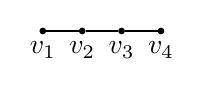
\begin{tikzpicture}[every node/.style={draw, circle, fill=black, minimum size=2pt, inner sep=0pt}]
\node[fill=black, label = below:$v_{1}$] (G1N2) at (6,4.5) {};
\node[fill=black, label = below:$v_{2}$] (G1N0) at (6.5,4.5) {};
\node[fill=black, label = below:$v_{3}$] (G1N1) at (7,4.5) {};
\node[fill=black, label = below:$v_{4}$] (G1N3) at (7.5,4.5) {};
\draw (G1N0) -- (G1N1);
\draw (G1N0) -- (G1N2);
\draw (G1N1) -- (G1N3);
\end{tikzpicture}
\end{document}
};
%        \node[anchor=east] (Lfile1) at (4.5,-2.5) {$(10,9,11)$};
        
%    \end{tikzpicture}
%    \caption{A $\sigma^{+-}$-labeling of $\mathbf{T_{6}^{6}} \sqcup \mathbf{T_{3}^{1}}\sim (4,1,8,5,6,7)\sqcup (10,9,11)$}
%    \label{fig:union_files}
%\end{figure}
    

%%%%%%%%%%%%%%%%%%%%%%%%%%%%%%%%%%%%%%%%%%%%%%%%%%%%%%%%%%%%%%%%%%%%%%%%%%%%%%%%%%%%%%%%%%%%%%%%%
\begin{figure}[H]
    \centering
    \begin{tikzpicture}[scale=0.5]
        %G1

        \node[anchor=east] (file1) at (0, 0) {\documentclass{standalone}
\usepackage{tikz}
\begin{document}
\begin{tikzpicture}[every node/.style={draw, circle, fill=black, minimum size=2pt, inner sep=0pt}]
\node[fill=black, label=above:{$v_{4}$}] (G1N1) at (90:0.5) {};
\node[fill=black, label=above left:{$v_{2}$}] (G1N0) at (90:0) {};
\node[fill=black, label=below right:{$v_{6}$}] (G1N2) at (306:0.5) {};
\node[fill=black, label=below left:{$v_{5}$}] (G1N3) at (234:0.5) {};
\node[fill=black, label=above left:{$v_{1}$}] (G1N4) at (162:0.5) {};
\node[fill=black, label=above right:{$v_{3}$}] (G1N5) at (18:0.5) {};
\draw (G1N0) -- (G1N1);
\draw (G1N0) -- (G1N2);
\draw (G1N0) -- (G1N3);
\draw (G1N0) -- (G1N4);
\draw (G1N0) -- (G1N5);
\end{tikzpicture}
\end{document}
};
        % Union symbol
        
        % Second standalone file
        \node[anchor=west] (file2) at (0.001, -0.62) {\documentclass{standalone}
\usepackage{tikz}
\begin{document}
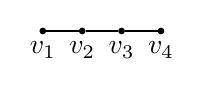
\begin{tikzpicture}[every node/.style={draw, circle, fill=black, minimum size=2pt, inner sep=0pt}]
\node[fill=black, label = below:$v_{1}$] (G1N2) at (6,4.5) {};
\node[fill=black, label = below:$v_{2}$] (G1N0) at (6.5,4.5) {};
\node[fill=black, label = below:$v_{3}$] (G1N1) at (7,4.5) {};
\node[fill=black, label = below:$v_{4}$] (G1N3) at (7.5,4.5) {};
\draw (G1N0) -- (G1N1);
\draw (G1N0) -- (G1N2);
\draw (G1N1) -- (G1N3);
\end{tikzpicture}
\end{document}
};

    \begin{scope}[shift={(3.75,0)}]
        \draw[dashed](0,1.75)--(0,-16.75);
    \end{scope}
%%%%%%%%%%%%%%%%%%%%%%%%%%%%%%%%% second column %%%%%%%%%%%%%%%%%%%%%%%%%%%%%%%%%%%%%%%%%%%%%%%%%

    \begin{scope}[shift = {(7.75,0)}]
        
        \node[anchor=east] (file1) at (0, 0) {\input{Danny's example/7 mod 14/1-T-(6,6)}};
        
        \node[anchor=west] (file2) at (0.001, -0.62) {\input{Danny's example/7 mod 14/1-T-(3,1)}};

        \draw[->] (4,0.01) -- (4,0.01) node[draw = none,midway, text=black, fill=white] {$\overset{+7}{\circlearrowright}$};
        %G2
        \node[anchor=east] (file1) at (0, -3) {\documentclass{standalone}
\usepackage{tikz}
\begin{document}
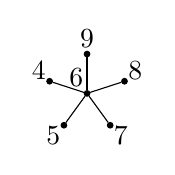
\begin{tikzpicture}[every node/.style={draw, circle, fill=black, minimum size=2pt, inner sep=0pt}]
\node[fill=black, label=above left:{$4$}] (G1N4) at (162:0.5) {};
\node[fill=black, label={[yshift=2pt]above left:{$6$}}] (G1N0) at (90:0) {};
\node[fill=black, label=above right:{$8$}] (G1N5) at (18:0.5) {};
\node[fill=black, label=above:{$9$}] (G1N1) at (90:0.5) {};
\node[fill=black, label=below left:{$5$}] (G1N3) at (234:0.5) {};
\node[fill=black, label=below right:{$7$}] (G1N2) at (306:0.5) {};
\draw (G1N0) -- (G1N1);
\draw (G1N0) -- (G1N2);
\draw (G1N0) -- (G1N3);
\draw (G1N0) -- (G1N4);
\draw (G1N0) -- (G1N5);
\end{tikzpicture}
\end{document}
};
        
        \node[anchor=west] (file2) at (0.001, -3.62) {\documentclass{standalone}
\usepackage{tikz}
\begin{document}
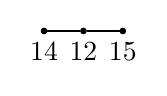
\begin{tikzpicture}[every node/.style={draw, circle, fill=black, minimum size=2pt, inner sep=0pt}]
\node[fill=black, label=below:{$14$}] (G1N1) at (6,4.5) {};
\node[fill=black, label=below:{$12$}] (G1N0) at (6.5,4.5) {};
\node[fill=black, label=below:{$15$}] (G1N2) at (7,4.5) {};
\draw (G1N0) -- (G1N1);
\draw (G1N0) -- (G1N2);
\end{tikzpicture}
\end{document}
};

        \draw[->] (4,-3.01) -- (4,-3.01) node[draw = none,midway, text=black, fill=white] {$\overset{+7}{\circlearrowright}$};
        %G3
        \node[anchor=east] (file1) at (0, -6) {\input{Danny's example/7 mod 14/3-T-(6,6)}};
        
        \node[anchor=west] (file2) at (0.001, -6.62) {\input{Danny's example/7 mod 14/3-T-(3,1)}};

        \draw[->] (4,-6.01) -- (4,-6.01) node[draw = none,midway, text=black, fill=white] {$\overset{+7}{\circlearrowright}$};
        %G4
        \node[anchor=east] (file1) at (0.246, -9) {\documentclass{standalone}
\usepackage{tikz}
\begin{document}
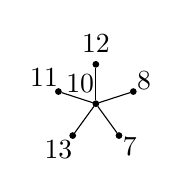
\begin{tikzpicture}[every node/.style={draw, circle, fill=black, minimum size=2pt, inner sep=0pt}]
\node[fill=black, label=above left:{$11$}] (G1N4) at (162:0.5) {};
\node[fill=black, label={[xshift=-0.5,yshift=2pt]above left:{$10$}}] (G1N0) at (90:0) {};
\node[fill=black, label=above right:{$8$}] (G1N5) at (18:0.5) {};
\node[fill=black, label=above:{$12$}] (G1N1) at (90:0.5) {};
\node[fill=black, label=below left:{$13$}] (G1N3) at (234:0.5) {};
\node[fill=black, label=below right:{$7$}] (G1N2) at (306:0.5) {};

\draw (G1N0) -- (G1N1);
\draw (G1N0) -- (G1N2);
\draw (G1N0) -- (G1N3);
\draw (G1N0) -- (G1N4);
\draw (G1N0) -- (G1N5);
\end{tikzpicture}
\end{document}};
        
        \node[anchor=west] (file2) at (0.001, -9.62) {\input{Danny's example/7 mod 14/4-T-(3,1)}};

        \draw[->] (4,-9.01) -- (4,-9.01) node[draw = none,midway, text=black, fill=white] {$\overset{+1}{\circlearrowright}$};

        %G5
        \node[anchor=east] (file1) at (0.246, -12) {\input{Danny's example/7 mod 14/5-T-(6,6)}};
        
        \node[anchor=west] (file2) at (0.001, -12.62) {\input{Danny's example/7 mod 14/5-T-(3,1)}};

        \draw[->] (4,-12.01) -- (4,-12.01) node[draw = none,midway, text=black, fill=white] {$\overset{+1}{\circlearrowright}$};
        \end{scope}
        
    \begin{scope}[shift={(12.9555,0)}]
        \draw[dashed](0,1.75)--(0,-16.75);
    \end{scope}
%%%%%%%%%%%%%%%%%%%%%%%%%%%%%%%%% third column %%%%%%%%%%%%%%%%%%%%%%%%%%%%%%%%%%%%%%%%%%%%%%%%%%
    \begin{scope}[shift={(17,0)}]

        %G1
        \node[anchor=east] (file1) at (0, 0) {\input{Danny's example/8 mod 14/1-T-(6,6)}};
        
        \node[anchor=west] (file2) at (0.001, -0.62) {\input{Danny's example/8 mod 14/1-T-(3,1)}};

        \draw[->] (4,0.01) -- (4,0.01) node[draw = none,midway, text=black, fill=white] {$\overset{+7}{\circlearrowright}$};
        %G2
        \node[anchor=east] (file1) at (0, -3) {\documentclass{standalone}
\usepackage{tikz}
\begin{document}
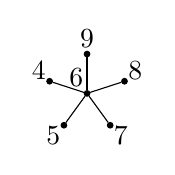
\begin{tikzpicture}[every node/.style={draw, circle, fill=black, minimum size=2pt, inner sep=0pt}]
\node[fill=black, label=above left:{$4$}] (G1N4) at (162:0.5) {};
\node[fill=black, label={[yshift=2pt]above left:{$6$}}] (G1N0) at (90:0) {};
\node[fill=black, label=above right:{$8$}] (G1N5) at (18:0.5) {};
\node[fill=black, label=above:{$9$}] (G1N1) at (90:0.5) {};
\node[fill=black, label=below left:{$5$}] (G1N3) at (234:0.5) {};
\node[fill=black, label=below right:{$7$}] (G1N2) at (306:0.5) {};
\draw (G1N0) -- (G1N1);
\draw (G1N0) -- (G1N2);
\draw (G1N0) -- (G1N3);
\draw (G1N0) -- (G1N4);
\draw (G1N0) -- (G1N5);
\end{tikzpicture}
\end{document}
};
        
        \node[anchor=west] (file2) at (0.001, -3.62) {\documentclass{standalone}
\usepackage{tikz}
\begin{document}
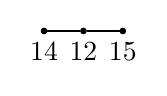
\begin{tikzpicture}[every node/.style={draw, circle, fill=black, minimum size=2pt, inner sep=0pt}]
\node[fill=black, label=below:{$14$}] (G1N1) at (6,4.5) {};
\node[fill=black, label=below:{$12$}] (G1N0) at (6.5,4.5) {};
\node[fill=black, label=below:{$15$}] (G1N2) at (7,4.5) {};
\draw (G1N0) -- (G1N1);
\draw (G1N0) -- (G1N2);
\end{tikzpicture}
\end{document}
};

        \draw[->] (4,-3.01) -- (4,-3.01) node[draw = none,midway, text=black, fill=white] {$\overset{+7}{\circlearrowright}$};
        %G3
        \node[anchor=east] (file1) at (0, -6) {\input{Danny's example/8 mod 14/3-T-(6,6)}};
        
        \node[anchor=west] (file2) at (0.001, -6.62) {\input{Danny's example/8 mod 14/3-T-(3,1)}};

        \draw[->] (4,-6.01) -- (4,-6.01) node[draw = none,midway, text=black, fill=white] {$\overset{+7}{\circlearrowright}$};
        %G4
        \node[anchor=east] (file1) at (0, -9) {\documentclass{standalone}
\usepackage{tikz}
\begin{document}
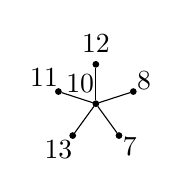
\begin{tikzpicture}[every node/.style={draw, circle, fill=black, minimum size=2pt, inner sep=0pt}]
\node[fill=black, label=above left:{$11$}] (G1N4) at (162:0.5) {};
\node[fill=black, label={[xshift=-0.5,yshift=2pt]above left:{$10$}}] (G1N0) at (90:0) {};
\node[fill=black, label=above right:{$8$}] (G1N5) at (18:0.5) {};
\node[fill=black, label=above:{$12$}] (G1N1) at (90:0.5) {};
\node[fill=black, label=below left:{$13$}] (G1N3) at (234:0.5) {};
\node[fill=black, label=below right:{$7$}] (G1N2) at (306:0.5) {};

\draw (G1N0) -- (G1N1);
\draw (G1N0) -- (G1N2);
\draw (G1N0) -- (G1N3);
\draw (G1N0) -- (G1N4);
\draw (G1N0) -- (G1N5);
\end{tikzpicture}
\end{document}};
        
        \node[anchor=west] (file2) at (0.001, -9.62) {\input{Danny's example/8 mod 14/4-T-(3,1)}};

        \draw[->] (4,-9.01) -- (4,-9.01) node[draw = none,midway, text=black, fill=white] {$\overset{+7}{\circlearrowright}$};
        
        %G5
        \node[anchor=east] (file1) at (0.246, -12) {\input{Danny's example/8 mod 14/5-T-(6,6)}};
        
        \node[anchor=west] (file2) at (0.001, -12.62) {\input{Danny's example/8 mod 14/5-T-(3,1)}};

        \draw[->] (4,-12.01) -- (4,-12.01) node[draw = none,midway, text=black, fill=white] {$\overset{+1}{\circlearrowright}$};

        %G6
        \node[anchor=east] (file1) at (0.246, -15) {\input{Danny's example/8 mod 14/6-T-(6,6)}};
        
        \node[anchor=west] (file2) at (0.001, -15.62) {\input{Danny's example/8 mod 14/6-T-(3,1)}};

        \draw[->] (4,-15.01) -- (4,-15.01) node[draw = none,midway, text=black, fill=white] {$\overset{+1}{\circlearrowright}$};

    \end{scope}
    \end{tikzpicture}
    \caption{A $\sigma^{+-}$-labeling of $F \cong\mathbf{T_{6}^{6}} \sqcup \mathbf{T_{3}^{1}}$ (left) and generating presentations for the $F$-decomposition of $K_{n}$ where $n=35$ (middle) and $n=36$ (right)}
    \label{fig:7mod14example}
\end{figure}
%%%%%%%%%%%%%%%%
\newpage
\section{$\mathbf{T_{7}^{11}}\sqcup\mathbf{T_{2}^{1}}$ -decompositions of $K_{n}$ for $n\equiv\,7,8\,\pmod{14}$} \label{sec:star}
%Danny

We begin this case by constructing $K_{n}$ for $n \equiv 7 \textrm{ or } 8 \pmod{14}$ and $n\geq 21$ using \textit{joined} copies of $K_{22}$, $K_{21}$, and $K_{14}$. Recall, the \textit{join} of two graphs $G_{1}$ and $G_{2}$ is the graph obtained by adding an edge $\{g_1,g_2\}$ for every vertex $g_1 \in V(G_{1})$ and every vertex of $g_2 \in V(G_{2})$.

Let $t$ be a positive integer and join $t-1$ copies of $K_{14}$ with each other and a lone copy of $K_{21}$. The resulting graph is $K_{14(t-1)+21} \cong K_{14t+7}$. So we can think of $K_{14t+7}$ as $K_{t}$ whose $t$ ``vertices'' consist of $t-1$ copies of $K_{14}$ and $1$ copy of $K_{21}$ and whose edges are the join between them. From now on, we will refer to these ``vertices'' as nodes. Similarly, $K_{14t+8}$ can be constructed as $K_{t}$ whose nodes are $t-1$ copies of $K_{14}$ and $1$ copy of $K_{22}$ and whose edges are the join between them.

We show that $\mathbf{T_{7}^{11}}\sqcup\mathbf{T_{2}^{1}}$ decomposes $K_{n}$ for $n\equiv7 \textrm{ or }8\pmod{14}$ by proving $K_{22},K_{21},K_{14},K_{22,14},K_{21,14},\text{ and }K_{14,14}$ are each $\mathbf{T_{7}^{11}}\sqcup\mathbf{T_{2}^{1}}$-decomposable. Notice that these 6 graphs make up the nodes and edges of the $K_{t}$ representations of $K_{14t+7}$ and $K_{14t+8}$ stated in the constructions above.

\noindent The proof of the next theorem was obtained by manipulating a $K_{1,7}$-decomposition of $K_{22}$ by Cain in \cite{bib:Cain}.

\begin{theorem}\label{thm:PCstarpath}
    $\mathbf{T_{7}^{11}}\sqcup\mathbf{T_{2}^{1}}$ decomposes $K_{21}$ and $K_{22}$.
\end{theorem}

\begin{proof}
     Figures 8 and 9 show $\mathbf{T_{7}^{11}}\sqcup\mathbf{T_{2}^{1}}$-decompositions of $K_{21}$ and $K_{22}$, respectively.  %The table will contain ad-hoc decompositions of $K_{21}$ and $K_{22}$. The construction for $K_{21}$ results from plucking edges off of Pauline Cain's $7$-star decomposition of $K_{21}$ and mixing them around, and The construction for $K_{22}$ results from adding three stars centered at $\infty$ and three lone paths beginning at $\infty$. Once again, edges are plucked off and mixed around to make this work.
\end{proof}

\begin{theorem} \label{thm:K_n,7}
    $\mathbf{T_{7}^{11}}\sqcup\mathbf{T_{2}^{1}}$ decomposes $K_{n,7}$ for all $n\geq 2$.
\end{theorem}

\begin{proof}
    Take the partite set of $n$ nodes to be $\ZZ_{n}$ and color them white. Then, take the other partite set of $7$ nodes to be $\ZZ_{7}$ and color them black. Notice that $|E(K_{n,7})|=|\ZZ_{n}\oplus \ZZ_{7}|=7n$. So let us refer to edges of $K_{n,7}$ as elements of $\ZZ_{n}\oplus \ZZ_{7}$ and vice versa. Note that since $n\geq 2, (1,0)\neq (0,0)$.
    \\
    
    \noindent Now, let $E_{i}= (i,0)+\{(0,0),(1,1),(1,2),\hdots,(1,6)\}$ for each $i\in \ZZ_{n}$ and $F_{i}$ be the subgraph induced by $E_{i}$. Since each $F_{i}$ contains a path $(i,0)$ which is vertex disjoint from the star centered at the white $i+1$, it must be isomorphic to $\mathbf{T_{7}^{11}}\sqcup\mathbf{T_{2}^{1}}$.
    \\
    %note to self: originally I thought of E_i's as (i,0) + (\{(0,0)\}\cup [(1,0)+[\langle (0,1)\rangle\setminus \{(0,0)\}]])

    %the union expression at the end is messy. However, the point of using groups here is basically that when we use generator notation we can swallow things up to get simpler things in terms of generators and it works out nicely here.
    
    \noindent Suppose that there exist distinct $i,j\in \ZZ_{n}$ such that $E_{i}\cap E_{j}\neq \emptyset$. But then we have that $(i,0)=(j,0)$ or $(i+1,a)=(j+1,b)$ for some $a,b\in \ZZ_{7}$, which is impossible. So all distinct $E_{i}$'s are pairwise disjoint, and therefore all distinct $F_{i}$'s are pairwise edge-disjoint. Lastly, $\bigcup_{i\in \ZZ_{n}} E_{i}=\langle (1,0)\rangle + [\{(0,0)\}\cup [(1,0)+\langle (0,1)\rangle] \setminus \{(1,0)\}]=\langle (1,0)\rangle + \langle (0,1)\rangle = \langle (1,0),(0,1)\rangle = \ZZ_{n}\oplus \ZZ_{7}$. Therefore, $\bigcup_{i\in \ZZ_{n}} F_{i} = K_{n,7}$. 
    \\
    
    \noindent Thus, $\{F_{i}\mid i\in \ZZ_{n}\}$ is a $\mathbf{T_{7}^{11}}\sqcup\mathbf{T_{2}^{1}}-$decomposition of $K_{n,7}$. Furthermore, This decomposition is generated by developing the white nodes of $F_{0}$ by $1$.
\end{proof}
\newpage
\begin{figure}
    \centering
    \input{starpath}
    \caption{A generating presentation of the $\mathbf{T_{7}^{11}}\sqcup\mathbf{T_{2}^{1}}$-decomposition of $K_{n,7}$}
    \label{fig:enter-label}
\end{figure}

\begin{cor}\label{cor:starpathbi}
    $\mathbf{T_{7}^{11}}\sqcup\mathbf{T_{2}^{1}}$ decomposes $K_{22,14}$, $K_{21,14},\text{ and }K_{14,14}$.
\end{cor}

\begin{proof}
    $\mathbf{T_{7}^{11}}\sqcup\mathbf{T_{2}^{1}}$ decomposes $K_{7,7}$ and $K_{8,7}$ by Theorem \ref{thm:K_n,7}. $K_{14,14}$ can be expressed as the edge-disjoint union of four copies of $K_{7,7}$, $K_{21,14}$ can be expressed as the edge-disjoint union of six copies of $K_{7,7}$, and $K_{22,14}$ can be expressed as the edge-disjoint union of two copies of $K_{8,7}$ and four copies of $K_{7,7}$. Therefore, $\mathbf{T_{7}^{11}}\sqcup\mathbf{T_{2}^{1}}$ decomposes them all.
\end{proof}

\begin{theorem}
$\mathbf{T_{7}^{11}}\sqcup\mathbf{T_{2}^{1}}$ decomposes $K_{14t+7}$ and $K_{14t+8}$ where $t$ is a positive integer. 
\end{theorem}
\begin{proof}
$\mathbf{T_{7}^{11}}\sqcup\mathbf{T_{2}^{1}}$ decomposes $K_{14}$ by Theorem \ref{thm:sigma plus minus}, $K_{22,14}$, $K_{21,14},\text{ and }K_{14,14}$ by Corollary \ref{cor:starpathbi}, and lastly $K_{22},K_{21}$ by Theorem \ref{thm:PCstarpath}.
\newline\newline
Therefore, $\mathbf{T_{7}^{11}}\sqcup\mathbf{T_{2}^{1}}$ decomposes the join of $(t-1)$ copies of $K_{14}$ with each other and $1$ copy of $K_{21}$, which is isomorphic to $K_{14t+7}$. Similarly $\mathbf{T_{7}^{11}}\sqcup\mathbf{T_{2}^{1}}$ decomposes the join of $(t-1)$ copies of $K_{14}$ with each other and $1$ copy of $K_{22}$ which is isomorphic to $K_{14t+8}$.
\end{proof}
%%%%%%%%%%
\newpage
\section{(1-2-3)-labelings and 1-rotational (1-2-3)-labelings}
%table: 7 (mod14)
\begin{figure}[H]
\centering
    \includegraphics[scale=0.9]{7(mod 14).pdf}
    \caption{(1-2-3)-labelings}
    \label{fig:7mod14}
\end{figure}
%table 8 (mod 14)
\newpage
\begin{figure}[H]
    \centering
    \includegraphics[scale=0.9]{8(mod 14).pdf}
    \caption{1-rotational (1-2-3)-labelings}
    \label{fig:8mod14}
\end{figure}
\newpage
\begin{figure}
\input{7(mod 14) pt 1}
\end{figure}
\newpage
\begin{figure}
\scalebox{1}{\input{7(mod 14) pt 2}}
\caption{(1-2-3)-labelings}
\end{figure}


\section{$\mathbf{T_{7}^{11}}\sqcup\mathbf{T_{2}^{1}}$-decompositions of $K_{21}$ and $K_{22}$}
%K21 chart
\begin{figure}[H]
    \documentclass{article}
\usepackage{tikz}
\usepackage{graphicx}  % For including external images
\usepackage{standalone}  % For including standalone files
\usepackage{youngtab}  % For tables
\usepackage{array}  % For \extrarowheight support
\usepackage{amsmath}
\usepackage{longtable}  % For multi-page tables
\usepackage{adjustbox}
\usepackage{float}
\usepackage{caption} % Allows captioning outside figures

\begin{document}

\begin{longtable}{|c|c|c|c|}
    \hline
    No. & Block & No. & Block \\
    \hline
    \endfirsthead

    \hline
    No. & Block & No. & Block \\
    \hline
    \endhead

    \hline
    \caption{A $\mathbf{T_{7}^{11}\sqcup T_{2}^{1}}$-decomposition of $K_{21}$}\\
    \endfoot
    
    \hline
    \caption{A $\mathbf{T_{7}^{11}\sqcup T_{2}^{1}}$-decomposition of $K_{21}$}\label{tab:starpathK21}\\
    \endlastfoot


    $1$  & $(15,14,16,17,18,19,20)\sqcup(0,2)$  & $2$  & $(13,15,16,17,18,19,20)\sqcup(0,6)$  \\
\hline
    $3$  & $(8,16,12,17,18,19,20)\sqcup(9,3)$  &     $4$  & $(8,17,9,11,18,19,20)\sqcup(16,0)$  \\
\hline
    $5$  & $(8,18,9,11,13,19,20)\sqcup(0,1)$  &     $6$  & $(8,19,10,11,12,13,20)\sqcup(0,15)$  \\
\hline
    $7$  & $(8,1,9,10,11,12,13)\sqcup(18,7)$  &     $8$  & $(1,2,9,10,11,12,13)\sqcup(14,7)$  \\
\hline
    $9$  & $(0,3,2,6,11,12,13)\sqcup(8,7)$  &     $10 $ & $(0,4,2,3,11,12,13)\sqcup(8,9)$  \\
\hline
    $11 $ & $(0,5,2,3,4,12,13)\sqcup(9,10)$  &     $12 $ & $(1,6,2,4,5,12,13)\sqcup(15,7)$  \\
\hline
    $13 $ & $(1,7,2,3,4,5,6)\sqcup(0,14)$  &     $14 $ & $(3,8,4,5,6,14,20)\sqcup(12,15)$  \\
\hline
    $15 $ & $(4,9,5,6,14,15,20)\sqcup(16,7)$  &     $16 $ & $(15,10,4,5,6,16,20)\sqcup(0,18)$  \\
\hline
    $17 $ & $(15,11,0,5,6,16,20)\sqcup(17,1)$  &     $18 $ & $(14,12,0,11,17,18,20)\sqcup(8,2)$  \\
\hline
    $19 $ & $(16,13,0,11,12,17,20)\sqcup(1,19)$  &     $20 $ & $(1,14,2,3,4,5,6)\sqcup(20,7)$  \\
\hline
    $21 $ & $(1,15,2,3,4,5,6)\sqcup(19,7)$  &     $22 $ & $(1,16,2,3,4,5,6)\sqcup(17,7)$  \\
\hline
    $23 $ & $(0,17,2,3,4,5,6)\sqcup(11,14)$  &     $24 $ & $(1,18,2,3,4,5,6)\sqcup(10,14)$  \\
\hline
    $25 $ & $(0,19,2,3,4,5,6)\sqcup(13,14)$  &     $26 $ & $(0,20,2,3,4,5,6)\sqcup(10,11)$  \\
\hline
    $27 $ & $(9,7,0,10,11,12,13)\sqcup(1,3)$  &     $28 $ & $(10,8,0,11,12,13,15)\sqcup(1,4)$  \\
\hline
    $29 $ & $(11,9,0,12,13,16,19)\sqcup(1,5)$  &     $30 $ & $(12,10,0,3,13,17,18)\sqcup(1,20)$ \\
\hline
%
\end{longtable}
\end{document}
    \caption{A $\mathbf{T_{7}^{11}}\sqcup\mathbf{T_{2}^{1}}$-decomposition of $K_{21}$}
    \label{fig:K21}
\end{figure}
%K22 chart
\begin{figure}[H]
    \documentclass{standalone}
\usepackage{tikz}
\usepackage{graphicx}  % For including external images
\usepackage{standalone}  % For including standalone files
\usepackage{youngtab}  % For tables
\usepackage{array}  % For \extrarowheight support
\usepackage{amsmath}
\usepackage{longtable}  % For multi-page tables

\begin{document}
\centering
\renewcommand{\arraystretch}{1.05} % Adjust row height multiplier (padding)
\resizebox{\textwidth}{!}{%
\begin{tabular}{|c|c|c|c|}
\hline
Element & Graph & Element & Graph \\
\hline
    $G_{1}$ & \begin{tabular}{@{}l@{}} $(15,14,16,17,18,19,20)\sqcup(0,2)$ \end{tabular} &     $G_{2}$ & \begin{tabular}{@{}l@{}} $(13,15,16,17,18,19,20)\sqcup(0,6)$ \end{tabular} \\
\hline
    $G_{3}$ & \begin{tabular}{@{}l@{}} $(8,16,12,17,18,19,20)\sqcup(9,3)$ \end{tabular} &     $G_{4}$ & \begin{tabular}{@{}l@{}} $(8,17,9,11,18,19,20)\sqcup(16,0)$ \end{tabular} \\
\hline
    $G_{5}$ & \begin{tabular}{@{}l@{}} $(8,18,9,11,13,19,20)\sqcup(0,1)$ \end{tabular} &     $G_{6}$ & \begin{tabular}{@{}l@{}} $(8,19,10,11,12,13,20)\sqcup(0,15)$ \end{tabular} \\
\hline
    $G_{7}$ & \begin{tabular}{@{}l@{}} $(8,1,9,10,11,12,13)\sqcup(6,\infty)$ \end{tabular} &     $G_{8}$ & \begin{tabular}{@{}l@{}} $(1,2,9,10,11,12,13)\sqcup(14,7)$ \end{tabular} \\
\hline
    $G_{9}$ & \begin{tabular}{@{}l@{}} $(0,3,2,6,11,12,13)\sqcup(8,7)$ \end{tabular} &     $G_{10}$ & \begin{tabular}{@{}l@{}} $(0,4,2,3,11,12,13)\sqcup(8,9)$ \end{tabular} \\
\hline
    $G_{11}$ & \begin{tabular}{@{}l@{}} $(0,5,2,3,4,12,13)\sqcup(9,10)$ \end{tabular} &     $G_{12}$ & \begin{tabular}{@{}l@{}} $(1,6,2,4,5,12,13)\sqcup(15,7)$ \end{tabular} \\
\hline
    $G_{13}$ & \begin{tabular}{@{}l@{}} $(1,7,2,3,4,5,6)\sqcup(13,\infty)$ \end{tabular} &     $G_{14}$ & \begin{tabular}{@{}l@{}} $(3,8,4,5,6,14,20)\sqcup(12,15)$ \end{tabular} \\
\hline
    $G_{15}$ & \begin{tabular}{@{}l@{}} $(4,9,5,6,14,15,20)\sqcup(16,7)$ \end{tabular} &     $G_{16}$ & \begin{tabular}{@{}l@{}} $(15,10,4,5,6,16,20)\sqcup(0,18)$ \end{tabular} \\
\hline
    $G_{17}$ & \begin{tabular}{@{}l@{}} $(15,11,0,5,6,16,20)\sqcup(17,1)$ \end{tabular} &     $G_{18}$ & \begin{tabular}{@{}l@{}} $(14,12,0,11,17,18,20)\sqcup(8,2)$ \end{tabular} \\
\hline
    $G_{19}$ & \begin{tabular}{@{}l@{}} $(16,13,0,11,12,17,20)\sqcup(1,19)$ \end{tabular} &     $G_{20}$ & \begin{tabular}{@{}l@{}} $(1,14,2,3,4,5,6)\sqcup(20,7)$ \end{tabular} \\
\hline
    $G_{21}$ & \begin{tabular}{@{}l@{}} $(1,15,2,3,4,5,6)\sqcup(19,7)$ \end{tabular} &     $G_{22}$ & \begin{tabular}{@{}l@{}} $(1,16,2,3,4,5,6)\sqcup(17,7)$ \end{tabular} \\
\hline
    $G_{23}$ & \begin{tabular}{@{}l@{}} $(0,17,2,3,4,5,6)\sqcup(11,14)$ \end{tabular} &     $G_{24}$ & \begin{tabular}{@{}l@{}} $(1,18,2,3,4,5,6)\sqcup(10,14)$ \end{tabular} \\
\hline
    $G_{25}$ & \begin{tabular}{@{}l@{}} $(0,19,2,3,4,5,6)\sqcup(13,14)$ \end{tabular} &     $G_{26}$ & \begin{tabular}{@{}l@{}} $(0,20,2,3,4,5,6)\sqcup(10,11)$ \end{tabular} \\
\hline
    $G_{27}$ & \begin{tabular}{@{}l@{}} $(9,7,0,10,11,12,13)\sqcup(20,\infty)$ \end{tabular} &     $G_{28}$ & \begin{tabular}{@{}l@{}} $(10,8,0,11,12,13,15)\sqcup(1,4)$ \end{tabular} \\
\hline
    $G_{29}$ & \begin{tabular}{@{}l@{}} $(11,9,0,12,13,16,19)\sqcup(1,5)$ \end{tabular} &     $G_{30}$ & \begin{tabular}{@{}l@{}} $(12,10,0,3,13,17,18)\sqcup(1,20)$ \end{tabular} \\
\hline
    $G_{31}$ & \begin{tabular}{@{}l@{}} $(0,\infty,1,2,3,4,5)\sqcup(18,7)$ \end{tabular} &     $G_{32}$ & \begin{tabular}{@{}l@{}} $(14,\infty,15,16,17,18,19)\sqcup(1,3)$ \end{tabular} \\
\hline
    $G_{33}$ & \begin{tabular}{@{}l@{}} $(7,\infty,8,9,10,11,12)\sqcup(0,14)$ \end{tabular} & & \\
\hline
\end{tabular}%
}
\end{document}
    \caption{A $\mathbf{T_{7}^{11}}\sqcup\mathbf{T_{2}^{1}}$-decomposition of $K_{22}$}
    \label{fig:K22}
\end{figure}
\newpage
%%%%%%%%%%%
\begin{thebibliography}{20}

\bibitem{bib:Cain}
P. Cain, 
Decomposition of complete graphs into stars, 
\textit{Bull. Austral. Math. Soc.} \textbf{10} (1974), 23--30.
\url{https://doi.org/10.1017/S0004972700040582}

 \bibitem{cyclicbipart}
S. I. El-Zanati, C. Vanden Eynden,
On the cyclic decomposition of complete graphs into bipartite graphs,
\textit{Australas. J. Combin.}, \textbf{24}, 2001, 209--219.

\bibitem{cyclic}
S. I. El-Zanati, C. Vanden Eynden,
On Rosa-type labelings and cyclic graph decompositions,
\textit{Math. Slovaca}, \textbf{59}, 2009, 1--18.

\bibitem{bib:Peters}
B. Freyberg, R. Peters, 
Decomposition of complete graphs into forests with six edges, 
\textit{Discuss. Math. Graph Theory}, In-press (34), (2024).

\bibitem{tran}
B. Freyberg, N. Tran, 
Decomposition of complete graphs into bipartite unicyclic graphs with eight edges, 
\textit{J. Combin. Math. Combin. Comput.}, \textbf{114}, (2020), 133--142.

\bibitem{seven}
D. Froncek, M. Kubesa, 
Decomposition of complete graphs into connected unicyclic bipartite graphs with seven edges,
\textit{Bull. Inst. Combin. Appl.}, \textbf{93}, (2021), 52--80.

\bibitem{bib:rosa}
A. Rosa,
On certain valuations of the vertices of a graph,
In: Theory of Graphs (Intl. Symp. Rome 1966), Gordon and Breach, Dunod, Paris,
1967, 349--355.

\end{thebibliography}


\end{document}

